\chapter{Elektromagnetische Wellen}

\section{Wellengleichung}

Bisher haben wir in der Elektrostatik und in unserer Betrachtung von stationären Strömen nur Fälle behandelt, bei denen galt:

\begin{equation*}
\rho(\vec{r})\neq 0,\; \vec{j}(\vec{r})\neq 0,\; \dot{\vec{E}}=0,\; \dot{\vec{B}}=0
\end{equation*}

Jetzt wollen wir elektromagnetische Wellen im Vakuum , also ohne Quellen, betrachten. Daher muss gelten: 

\begin{equation*}
\rho=0,\; \vec{j}=0,\; \dot{\vec{E}}\neq 0,\; \dot{\vec{B}}\neq 0
\end{equation*}

Daraus folgt zunächst für die \textsc{Maxwell}-Gleichungen:

\begin{align*}
\div \vec{E} &=0 &\div \vec{B} &= 0\\
\rot  \vec{E} &= -\dot{\vec{B}} &\rot \vec{B} &= \epsilon_0\mu_0 \dot{\vec{E}}\\
\end{align*}

\begin{align*}
\Rightarrow\qquad & \rot\dot{\vec{B}} = \epsilon_0\mu_0\ddot{\vec{E}} = -\rot\rot\vec{E} = -\nabla\underbrace{(\nabla\cdot\vec{E})}_{\div\vec{E}=0} \ + \ \nabla^2 \vec{E}\\
\ \\
\overset{\epsilon_0\mu_0 = \frac{1}{c^2}}{\Rightarrow} \quad \alignedbox{}{\hphantom{a}\left(\frac{1}{c^2} \ \pddiff{}{t} \ - \ \laplace\right)\vec{E} \ =: \ \Dalembert\vec{E} \ = \ 0\hphantom{a}}
\end{align*}

Die erhaltene partielle Differentialgleichung ist die sogenannte \textbf{Wellengleichung}, welche sich auch analog für das $\vec{B}$-Feld herleiten lässt. Das Symbol $\Dalembert$ wird auch als \textbf{Wellen-} oder \textbf{\textsc{D'Alembert}-Operator} bezeichnet.


\section{Lösungen der Wellengleichung}

$\Dalembert U = 0$

\begin{enumerate}
\item \textbf{eindimensionale Lösung} ($\vec{r}\  \rightarrow \ x$)
\begin{equation*}
\left(\frac{1}{c^2} \ \pddiff{}{t} \ - \ \pddiff{}{x}\right)\ U(x,t) \ = \ 0 \ = \ \left(\frac{1}{c}\ \partial_t \ + \ \partial_x\right)\left(\frac{1}{c} \ \partial_t \ - \ \partial_x\right) \ U(x,t)
\end{equation*}

\begin{enumerate}
\item $\left(\frac{1}{c}\partial_t+\partial_x\right)U(x,t) = 0 \quad\Rightarrow\quad \partial_t U = - \ c \partial_x U \quad\Rightarrow\quad U = (u_1(x-ct))$
\item $\left(\frac{1}{c}\partial_t-\partial_x\right)U(x,t) = 0 \quad\Rightarrow\quad \partial_t U =\quad c \partial_x U \quad\Rightarrow\quad U = (u_2(x+ct))$
\end{enumerate}

mit zwei beliebigen Funktionen $u_1,u_2$, welche gegebene Anfangsbedingungen $U(t=0,x) \ , \ \partial_t U(t=0,x)$ der vollständigen Lösung erfüllen:

\begin{equation*}
U \ = \ u_1(x\ -\ ct) + u_2(x\ +\ ct)
\end{equation*}

\item
\textbf{Harmonische Welle}\\
\ \\
Exponentialansatz:

\begin{align*}
& U=U_0 e^{ik_x x}e^{ik_y y}e^{ik_z z}e^{-i\omega t} = U_0 e^{i(\vec{k}\vec{r}-\omega
t)}\\
\ \\
\overset{\text{Einsetzen}}{\Rightarrow} &\quad\Dalembert U = \left(\frac{1}{c^2} \ \pddiff{}{t} \ - \ \laplace\right)U = \left[\left(\frac{-i\omega}{c}\right)^2 \ - \ \left(i\vec{k}\right)^2\right]U = 0\\
\Rightarrow \ \quad&\qquad \omega^2 \ = \ c^2 \vec{k}^2
\end{align*}

Die Abhängigkeit $\omega(\vec{k})$ bezeichnet man als \textbf{Dispersionsrelation}. Für den Spezialfall $\vec{k} = k \cdot \vec{e}_x$ erhält man:

\begin{equation*}
U \ = \ U_0 \ e^{i(kx \ - \ \omega t)} \ = \ \underbrace{U_0 \ e^{ik\left(x-\frac{\omega}{k}t\right)} }_{(*)}
\end{equation*}

$(*)$ ist dabei der Spezialfall $u_1(x-ct)$, wie er in i) behandelt wurde.\\
Daraus folgt für die Ausbreitungsgeschwindigkeit $c =\frac{\omega}{|\vec{k}|}$ mit $|\vec{k}|=\frac{2\pi}{\lambda}$, welche in diesem Zusammenhang auch \textbf{Phasengeschwindigkeit} genannt wird.\\
Die Harmonische Welle breitet sich mit ebenjener Geschwindigkeit in Richtung $\vec{e}_k := \frac{\vec{k}}{|\vec{k}|}$ aus.

\item \textbf{Allgemeine Lösung}

\begin{equation*}
U(\vec{r},t) \ = \ \operatorname{Re} \left(\int\mathrm{d}^3 k \; U(\vec{k}) \ e^{i(\vec{k}\vec{r} \ - \ \omega t)}\right)
\end{equation*}

mit $\omega = \omega(\vec{k}) = |\vec{k}| \cdot c$\\
Man hat somit wieder zwei freie Funktionen $\operatorname{Re}(U(\vec{k})),\; \operatorname{Im}(U(\vec{k}))$ für zwei reelle Anfangsbedingungen $U(\vec{r},t=0),\ \partial_t U(\vec{r},t=0)$

\end{enumerate}


\section{Polarisation}
\begin{wrapfigure}[]{r}[0cm]{0cm}
	\raisebox{0pt}[\dimexpr\height-1\baselineskip\relax]{
		\colorbox{hgrey}{
			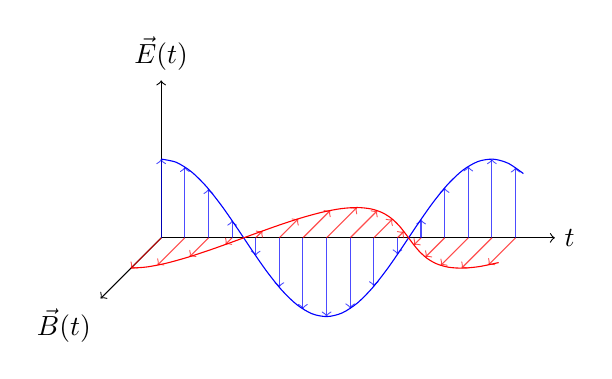
\begin{tikzpicture}
			
			\draw[->] (0,0,0)-- (5,0,0) node[right]{$t$};
			\draw[->] (0,0,0)-- (0,2,0) node[above]{$\vec{E}(t)$};
			\draw[->] (0,0,0)-- (0,0,2) node[below left]{$\vec{B}(t)$};
			
			\draw[scale=1,domain=0:4.6,smooth,variable=\t,blue] plot ({\t},{cos(1.5*deg(\t))},{0});
			\foreach \t in{0,0.3,...,4.6}{
				\draw[color=blue, opacity=0.7,->]
				(\t,0,0) -- ({\t},{cos(1.5*deg(\t))},{0});
			}
			
			\draw[scale=1,domain=0:4.6,smooth,variable=\t,red] plot ({\t},{0},{cos(1.5*deg(\t))});
			\foreach \t in{0,0.3,...,4.6}{
				\draw[color=red, opacity=0.7,->]
				(\t,0,0) -- ({\t},{0},{cos(1.5*deg(\t))});
			}
			
			
			\end{tikzpicture}
		}
	}
	\caption{elektromagnetische Welle}
\end{wrapfigure}
Betrachte die spezielle Lösung $\vec{E}_0 \cdot e^{i(\vec{k}\vec{r} - \omega t)}$ der Wellengleichung $\Dalembert \vec{E} = 0$. Bisher haben wir die Richtung von $\vec{E}_0$ beliebig angesehen. Dennoch gilt nach den \textsc{Maxwell}-Gleichungen:\
\\
\ \\ \linebreak\linebreak\linebreak\linebreak
\underline{$\div\vec{E} = 0$:}

\begin{equation*}
\div \vec{E} = i\vec{k}\cdot\vec{E}_0 \cdot e^{i(\vec{k}\vec{r} - \omega t)} \overset{!}{=} 0 \quad \Rightarrow \quad \text{\colorbox{bblue}{$\hspace{.5em}\vec{k}\perp\vec{E}\hspace{.5em}$\vphantom{\big|}}}
\end{equation*}
\ \\

\underline{$\rot\vec{E} = - \dot{\vec{B}}$}

\begin{align*}
\rot\vec{E} = i\vec{k}\times\vec{E} \overset{!}{=} i \omega\vec{B} \quad \Rightarrow \quad &\vec{e}_k\times\vec{E} = \frac{\omega}{k}\vec{B}\\
\Rightarrow\quad\vec{e}_k\times\vec{E} = c \cdot\vec{B} \quad\Rightarrow \quad \alignedbox{}{\hspace{.5em}\vec{B} \perp \vec{k}\hspace{.5em}\vphantom{\big|}}
\end{align*}

Daraus folgt, dass elektromagnetische Wellen transversal sind.\

Nun kann man noch zwei Fälle für den Vektor $\vec{E}_0$ bzw. $\vec{B}_0$ unterscheiden:

\begin{enumerate}

\item $ \quad \vec{E}_0$ ist reell

\begin{equation*}
\vec{E} = \operatorname{Re} \vec{E}_0 \cdot e^{i(\vec{k}\vec{r}-\omega t)} = \vec{E}_0 \cos(\vec{k}\vec{r}-\omega t) 
\end{equation*}

Für einen reellen Wert für $\vec{E}_0$ spricht man von \textbf{linearer Polarisation} der Welle.

\item $\quad \vec{E}_0$ ist komplex\\
\ \\
$\vec{E}_0 =\vec{E}_1 + i\vec{E}_2$ wobei $\{\vec{E}_1,\vec{E}_2 \}\perp\vec{k}$ und reell.

\begin{equation*}
\vec{E} = \vec{E}_0 \ e^{i(\vec{k}\vec{r}-\omega t)} = \vec{E}_1 \ \cos(\vec{k}\vec{r}-\omega t) \ - \ \vec{E}_2 \sin (\vec{k}\vec{r} - \omega t)
\end{equation*}

Es handelt sich im Endeffekt um zwei linear polarisierte Wellen mit einer Phasenverschiebung. Wir betrachten diese nun an einem festen Ort $\vec{r}$ und unterscheiden mehrere Fälle:

\begin{enumerate}
\item $\vec{E}_1\parallel\vec{E}_2\parallel\vec{e} \quad $ mit $\vec{e}$ Einheitsvektor in Richtung von $\vec{E}_1$ und $\vec{E}_2$

\begin{align*}
\vec{E} \ = \ \vec{e} \ (E_1 \ \cos \omega t \ + \ E_2 \ \sin \omega t) \  = \  \vec{e}  \ E' \ \cos(\omega t + \phi)\\
\Rightarrow \qquad \text{ linear polarisiert}
\end{align*}

\item $\vec{E}_1\perp\vec{E}_2 \qquad$ (setze: $\vec{E}_1\parallel\vec{e}_x, \  \vec{E}_2\parallel\vec{e}_y, \  \vec{k}\parallel\vec{e}_z$)

\begin{equation*}
\vec{E} \ = \ E_1 \ \vec{e}_x \ \cos \omega t \; + \; E_2 \ \vec{e}_y \ \sin\omega t
\quad\Rightarrow \quad \textbf{ elliptisch polarisiert}
\end{equation*}

Speziell: $ \; |\vec{E}_1| \ = \ |\vec{E}_2| $

\begin{equation*}
\vec{E_1} \; = \; \begin{cases}
					\quad \vec{E}_2 \qquad \textbf{links zirkular polarisiert}\\
					- \; \vec{E}_2 \qquad \textbf{rechts zirkular polarisiert}
				  \end{cases}	
\end{equation*}

\item $\vec{E}_1\nparallel\vec{E}_2, \ \vec{E}_1 \not\perp \vec{E}_2$\\
\ \\
ebenfalls elliptisch polarisiert

\end{enumerate}
\end{enumerate}